%% The 3W Well Data Viewer at the 5th Workshop on the 3W.
%%
%% Build: `latexmk` in this folder (see latexmkrc and README.md). The look is
%% the workshop's PowerPoint template, reproduced by beamerthemews3w.sty; the
%% screenshots are the ones of docs/assets/, so retaking them (scripts/
%% screenshots.py) refreshes the deck too. Fifteen minutes: about one minute a
%% frame, the title and the closing frame taking seconds.

\documentclass[aspectratio=169, 10pt, t]{beamer}
\usetheme{ws3w}

\usepackage{array}
\usepackage{booktabs}
\usepackage{qrcode}
\hypersetup{colorlinks=true, urlcolor=ws3wblue, linkcolor=ws3wnavy}

\newcolumntype{L}[1]{>{\raggedright\arraybackslash}p{#1}}

\title{3W Well Data Viewer}
\subtitle{A desktop GUI to inspect the real instances of the 3W dataset}
\author{Thiago Tom\'as de Paula}
\institute{Your affiliation}  % TODO: fill in before sending
\date{5th Workshop on the 3W \\ November 2026}

\begin{document}

\wstitleframe

% ---------------------------------------------------------------------------
\begin{frame}{Why a viewer for the real instances?}
  \begin{columns}[T]
    \begin{column}{0.55\textwidth}
      \begin{itemize}
        \item 3W 2.0.0 ships \textbf{1,119 real instances} on \textbf{40 wells}; 986 of them
          overlap another instance of their well in time. One stretch of a well can be
          filed twice, under two labels.
        \item Every file carries every column the dataset declares. \textbf{What each sensor
          actually recorded} is a question of its own: the downhole pressure is frozen in
          more than half of the real instances.
        \item The literature answers such questions with figures \textbf{drawn by hand}, one
          well or one fault at a time, from a sample of the instances.
        \item The viewer draws them \textbf{live, over every real instance}, the time series
          of any instance one click away. It trains no model: it is a lens on the data as
          3W ships it.
      \end{itemize}
    \end{column}
    \begin{column}{0.42\textwidth}
      \footnotesize
      \begin{tabular}{@{}L{0.56\linewidth}L{0.36\linewidth}@{}}
        \toprule
        Drawn by hand in the literature & Drawn live, on the page \\
        \midrule
        The instances of a well along time & \wspage{Timelines} \\
        Availability maps of the sensors & \wspage{Availability} \\
        Instances of one fault side by side & \wspage{Faults}, \wspage{Features} \\
        One variable against another & \wspage{Dispersions} \\
        Fixed-size, one-label windows, as a model reads them & \wspage{Windows} \\
        Clusterings and one-class models of the instances & \wspage{Instances} \\
        The Toolkit's \texttt{CleanSignals} rule & \wspage{Availability}, \wspage{Timelines} \\
        \bottomrule
      \end{tabular}
    \end{column}
  \end{columns}
\end{frame}

% ---------------------------------------------------------------------------
\begin{frame}{Seven pages, one question each}
  \begin{columns}[T]
    \begin{column}{0.66\textwidth}
      \small
      \begin{tabular}{@{}lL{0.78\linewidth}@{}}
        \toprule
        Page & Question \\
        \midrule
        \wspage{Timelines}    & How do the instances and the fault classes of each well spread out across time? \\
        \wspage{Availability} & What did each sensor actually record, beyond what the file declares? \\
        \wspage{Faults}       & How does one fault look on every well it occurred on? \\
        \wspage{Features}     & What does one sensor read under every fault class? \\
        \wspage{Dispersions}  & How do two sensors move together, and how much of it is the historian's interpolation? \\
        \wspage{Windows}      & What does a model see: one sensor of a well in fixed-size windows, one label each? \\
        \wspage{Instances}    & Where does every real instance sit on one plane, by what its sensors amount to? \\
        \bottomrule
      \end{tabular}
      \vskip 3mm
      A click on any bar, cell, point or plot opens the \textbf{instance window} of that
      instance and of every instance it overlaps. \texttt{F1} anywhere opens the Help.
    \end{column}
    \begin{column}{0.31\textwidth}
      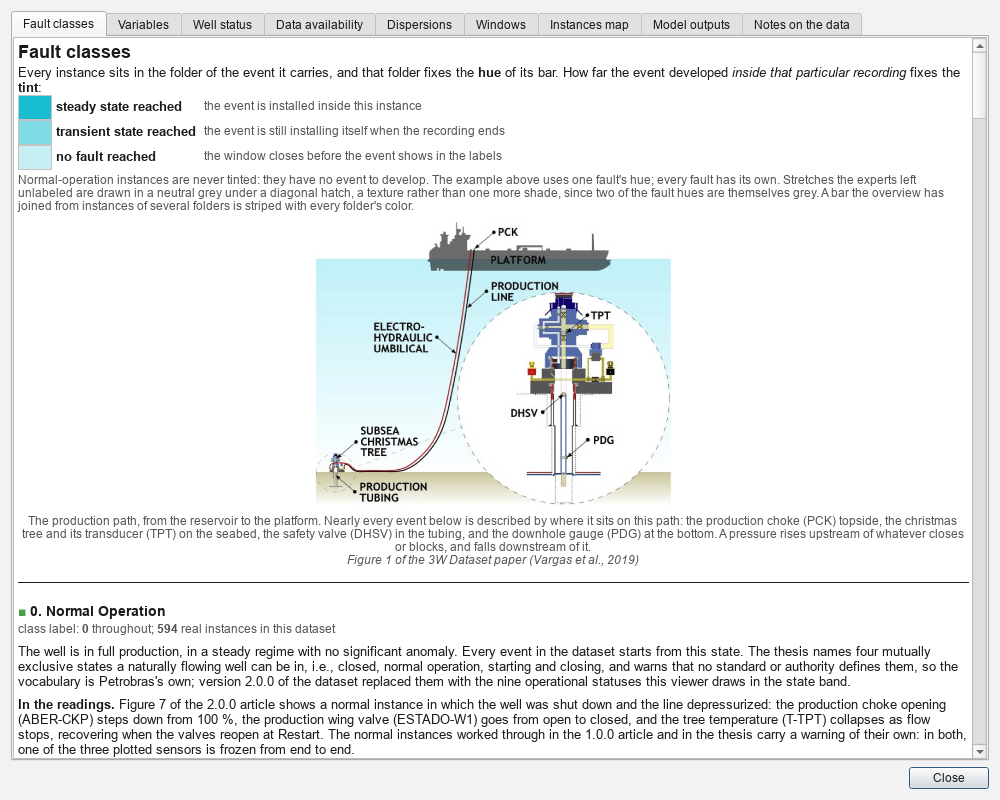
\includegraphics[width=\linewidth]{../assets/help.png}
      {\scriptsize\color{ws3wbrown} The Help: the platform and its sensors, the fault classes
      and their signatures, the well statuses, the data availability, the sources.\par}
    \end{column}
  \end{columns}
\end{frame}

% ---------------------------------------------------------------------------
\begin{frame}{Timelines: every real instance of every well}
  \begin{columns}[T]
    \begin{column}{0.6\textwidth}
      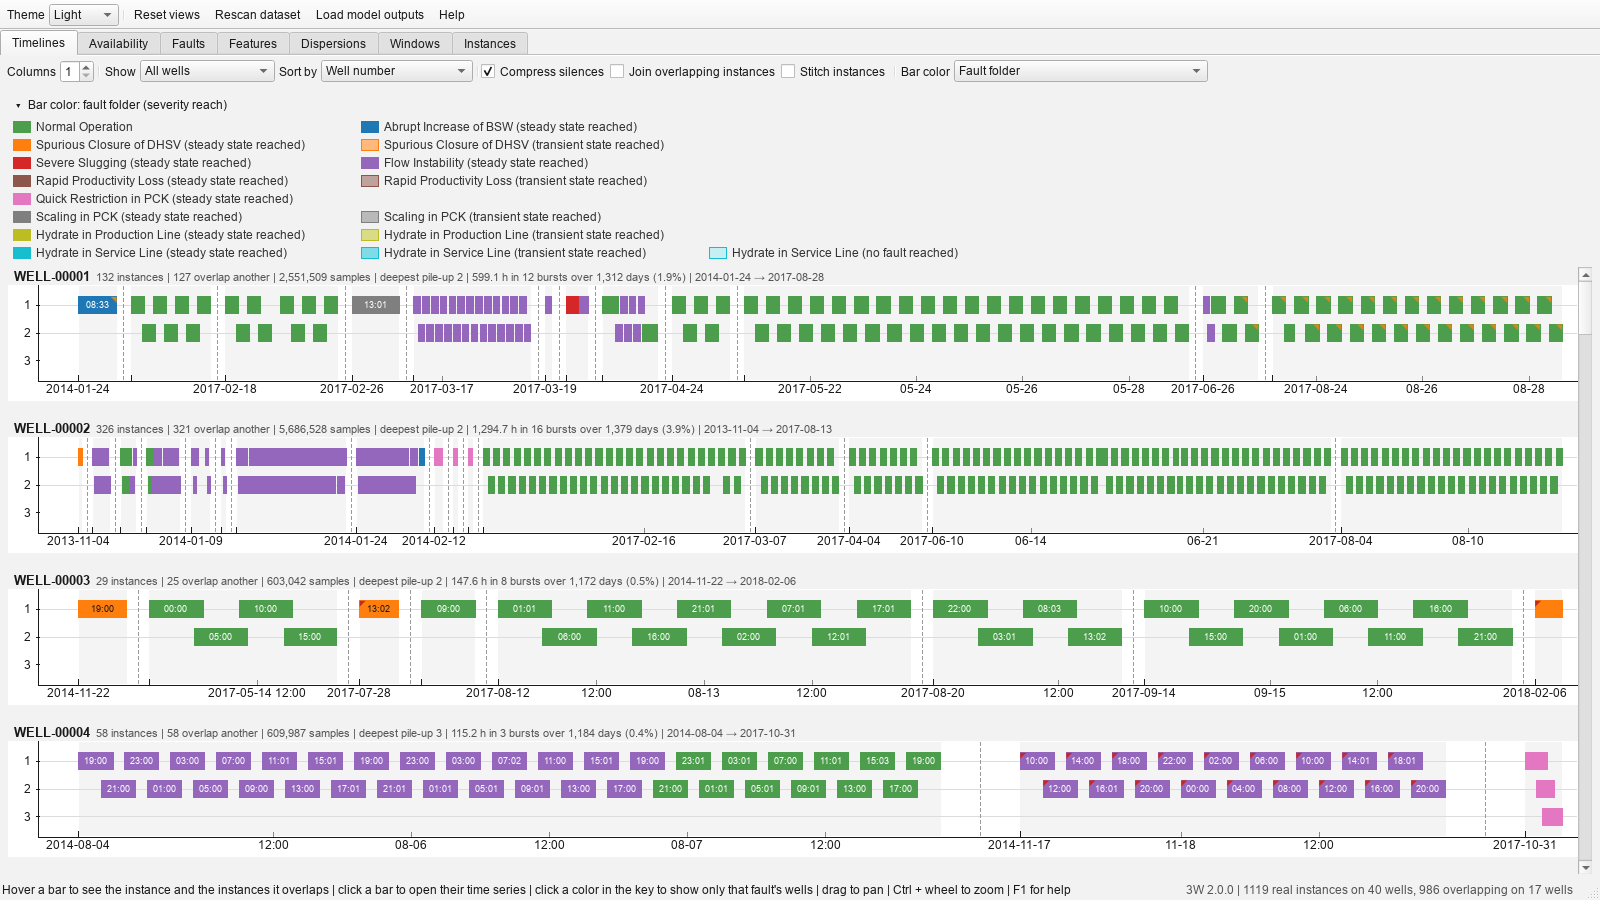
\includegraphics[width=\linewidth]{../assets/overview.png}
    \end{column}
    \begin{column}{0.38\textwidth}
      \footnotesize
      \begin{itemize}
        \item One timeline per well; every instance a bar from its first to its last
          timestamp, \textbf{stacked where it overlaps} another.
        \item \textbf{Join overlapping instances} merges the bars whose labels agree, so what
          still overlaps is exactly the labeling conflicts. \textbf{Stitch} lays a well's
          recordings end to end.
        \item \textbf{Bar color}: the fault folder, a sensor's availability or measurements,
          a descriptor, what the Toolkit's \texttt{CleanSignals} keeps, the agreement with
          model outputs.
        \item Hover names an instance and its partners; a click opens the instance window.
      \end{itemize}
    \end{column}
  \end{columns}
\end{frame}

% ---------------------------------------------------------------------------
\begin{frame}{Availability: what each sensor actually recorded}
  \begin{columns}[T]
    \begin{column}{0.41\textwidth}
      \footnotesize
      \begin{itemize}
        \item \textbf{Sensor availability}: per sensor and group of instances, the share
          \textbf{live}, \textbf{frozen} or \textbf{absent}. A frozen gauge is not available.
        \item \textbf{Sensor pairs}: how often two sensors carry a reading at the same
          instant. 102 of the 351 pairs never do.
        \item \textbf{Sensor correlations}: Pearson, mutual information and the nonlinear
          part, summed into Melo's global coefficient.
        \item The Toolkit's \texttt{CleanSignals} applied on the fly, thresholds movable: the
          cells it would discard are slashed, the columns it would drop greyed.
        \item \textbf{Corner marks}: an implausible reading (amber), pressures out of order
          (amber), a well status its valves contradict (red).
      \end{itemize}
    \end{column}
    \begin{column}{0.57\textwidth}
      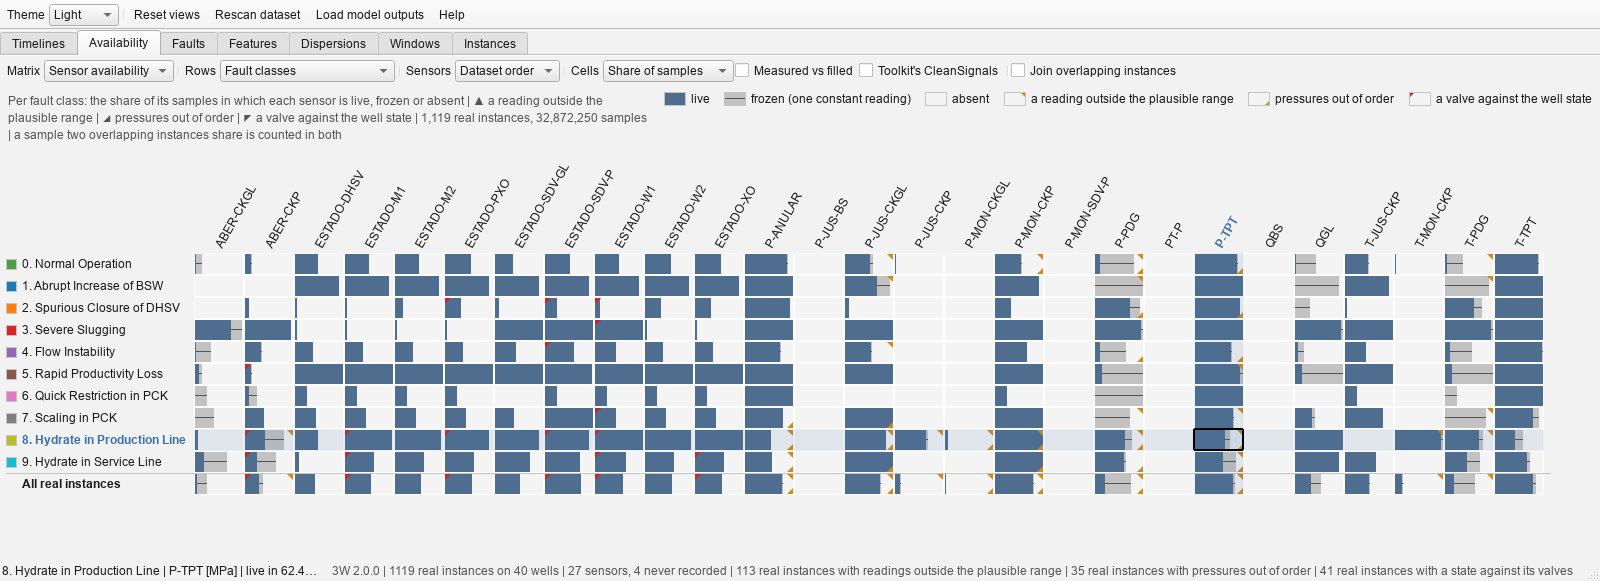
\includegraphics[width=\linewidth]{../assets/availability.png}
      \vskip 2mm
      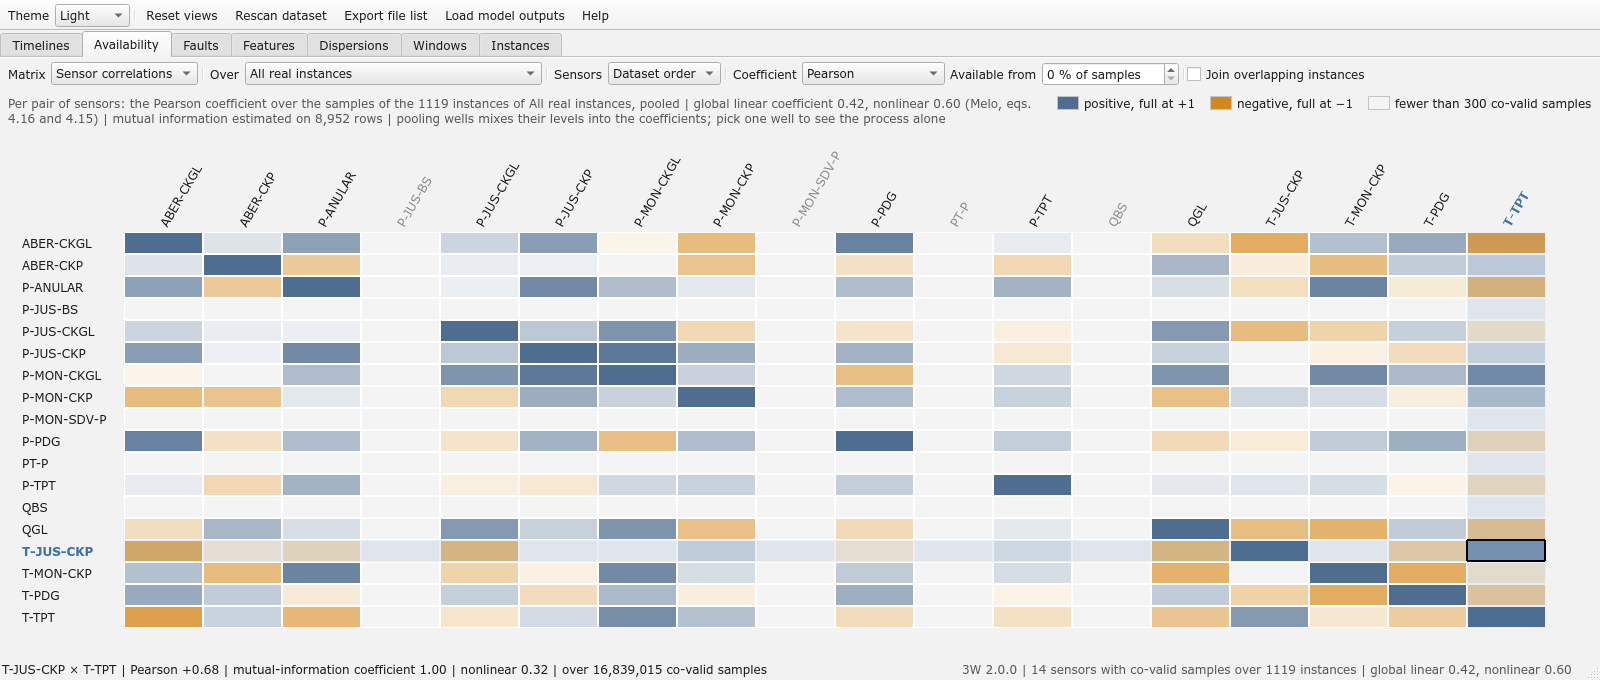
\includegraphics[width=0.72\linewidth]{../assets/correlations.png}
    \end{column}
  \end{columns}
\end{frame}

% ---------------------------------------------------------------------------
\begin{frame}{Faults and Features: across wells, across events}
  \begin{center}
    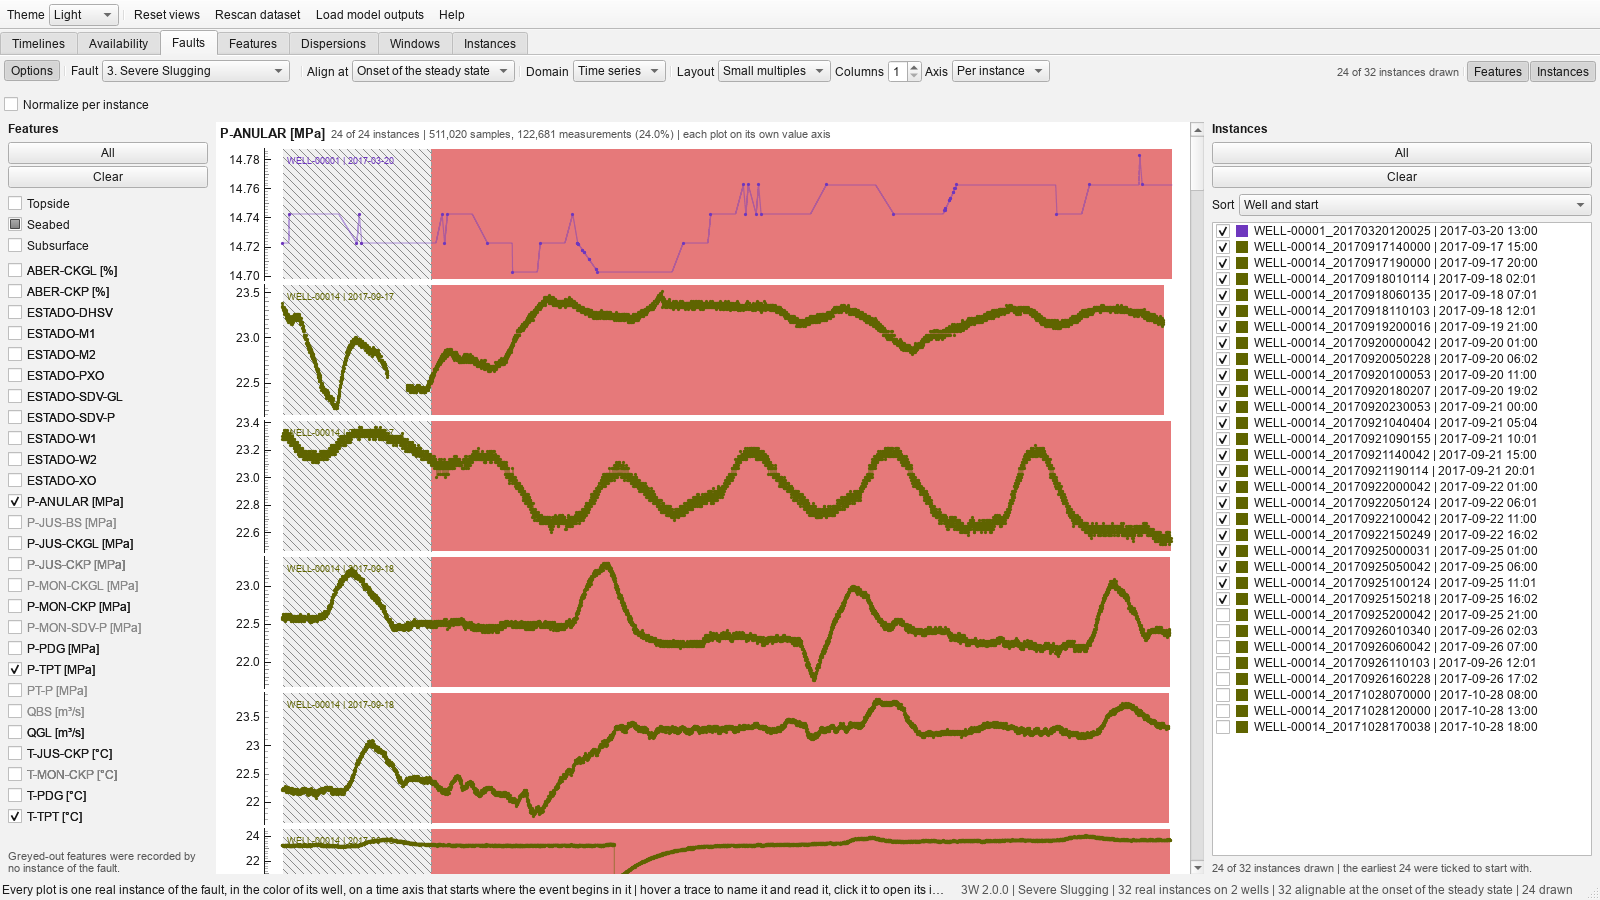
\includegraphics[width=0.44\textwidth]{../assets/faults.png}\hspace{4mm}
    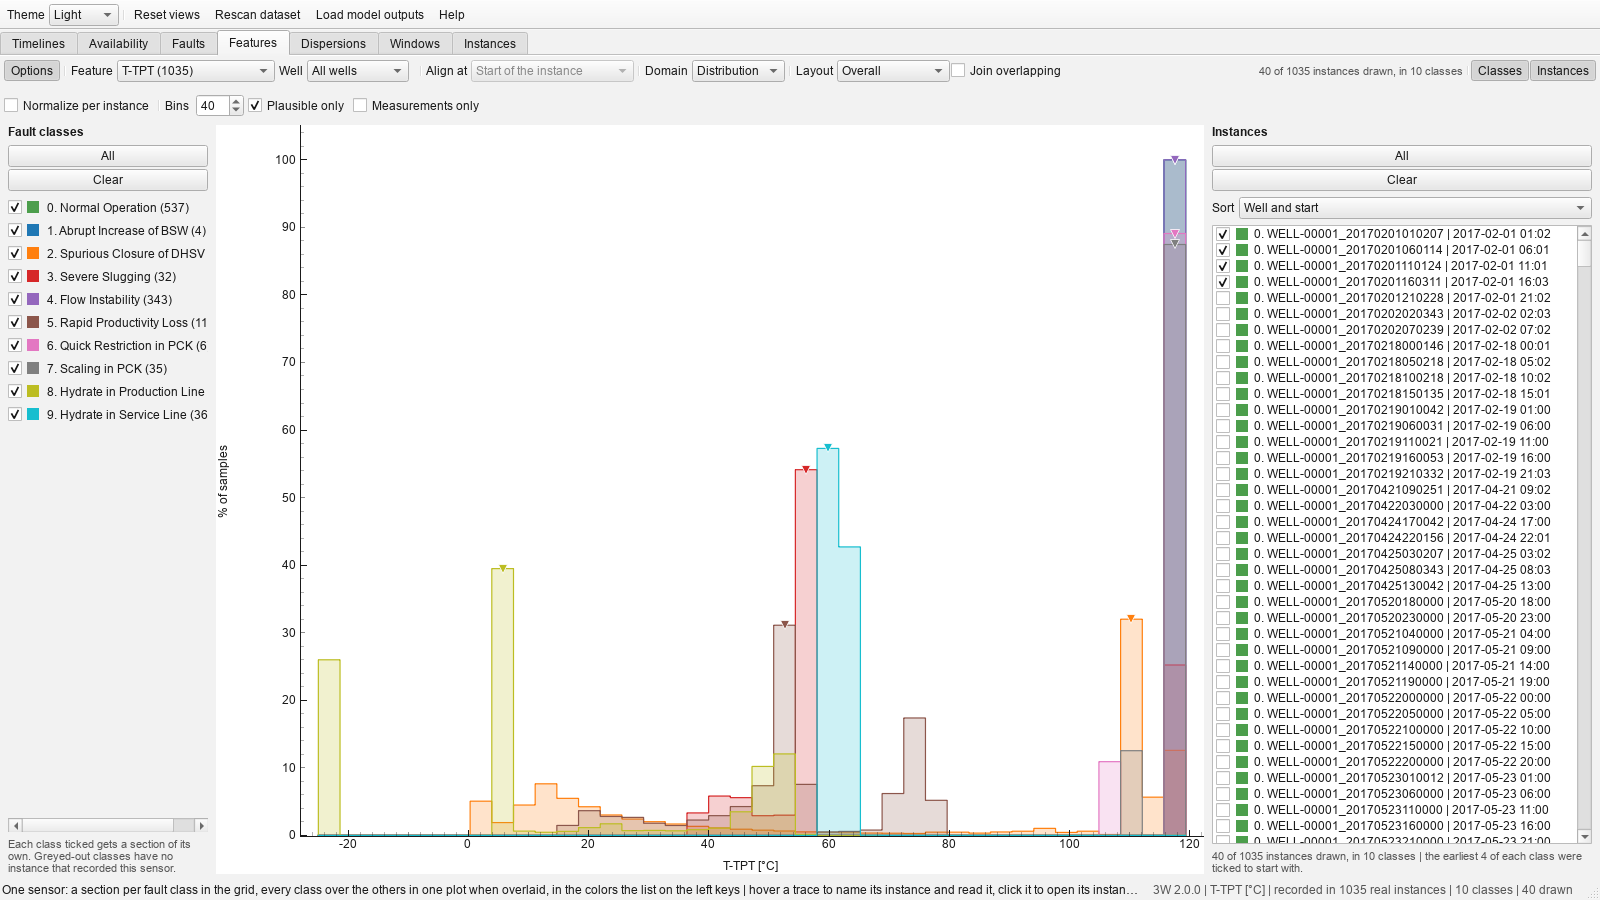
\includegraphics[width=0.44\textwidth]{../assets/features.png}
  \end{center}
  \vskip -1mm
  \footnotesize
  \begin{itemize}
    \item \wspage{Faults}: every real instance of one fault, from every well, \textbf{aligned
      at the onset} of the event, one section per sensor, one color per well.
    \item \wspage{Features}: the question turned round: one sensor, one section per fault
      class, so what a gauge reads under a hydrate sits beside what it reads under slugging.
    \item Both: small multiples or overlaid; the \textbf{time}, \textbf{distribution} or
      \textbf{spectrum} domain (Welch on the grid, Lomb-Scargle on the measurements alone);
      z-scores per instance; the label periods shaded behind every trace.
  \end{itemize}
\end{frame}

% ---------------------------------------------------------------------------
\begin{frame}{Dispersions and Windows: two more views}
  \begin{columns}[T]
    \begin{column}{0.48\textwidth}
      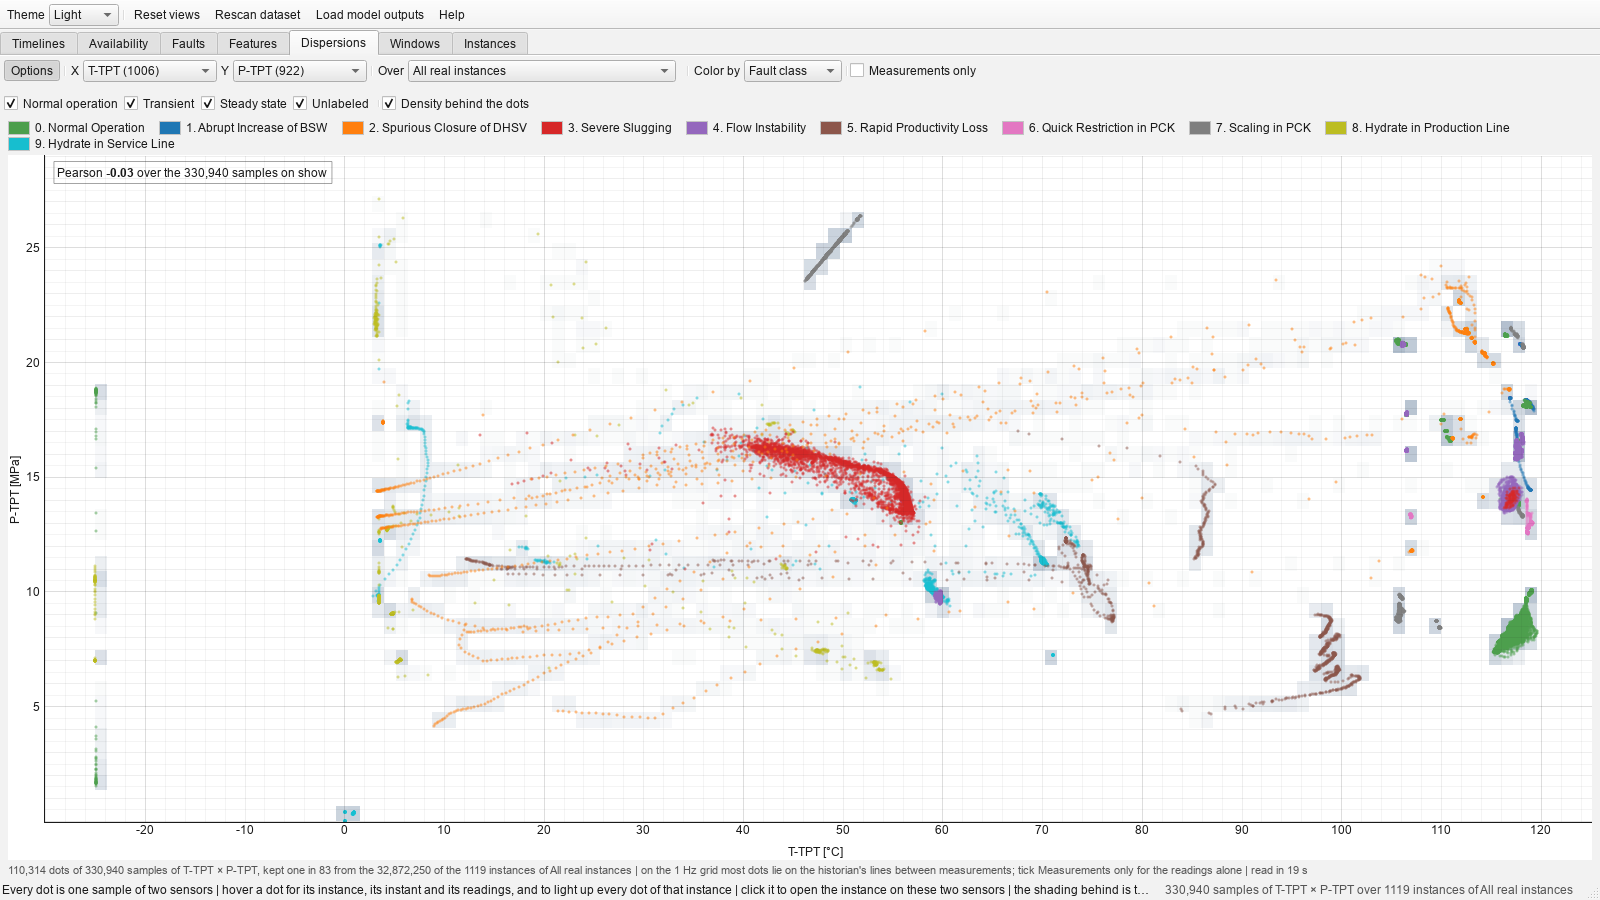
\includegraphics[width=\linewidth]{../assets/dispersion.png}
      \vskip 1.5mm
      \footnotesize
      \begin{itemize}
        \item \wspage{Dispersions}: two sensors against each other, every sample a dot over
          its density, colored by class, well or label period.
        \item \textbf{Measurements only} keeps the instants at which both were read: under
          severe slugging P-TPT against T-TPT reads $+0.40$ over every sample and $+0.95$
          over the 5\,\% measured.
      \end{itemize}
    \end{column}
    \begin{column}{0.48\textwidth}
      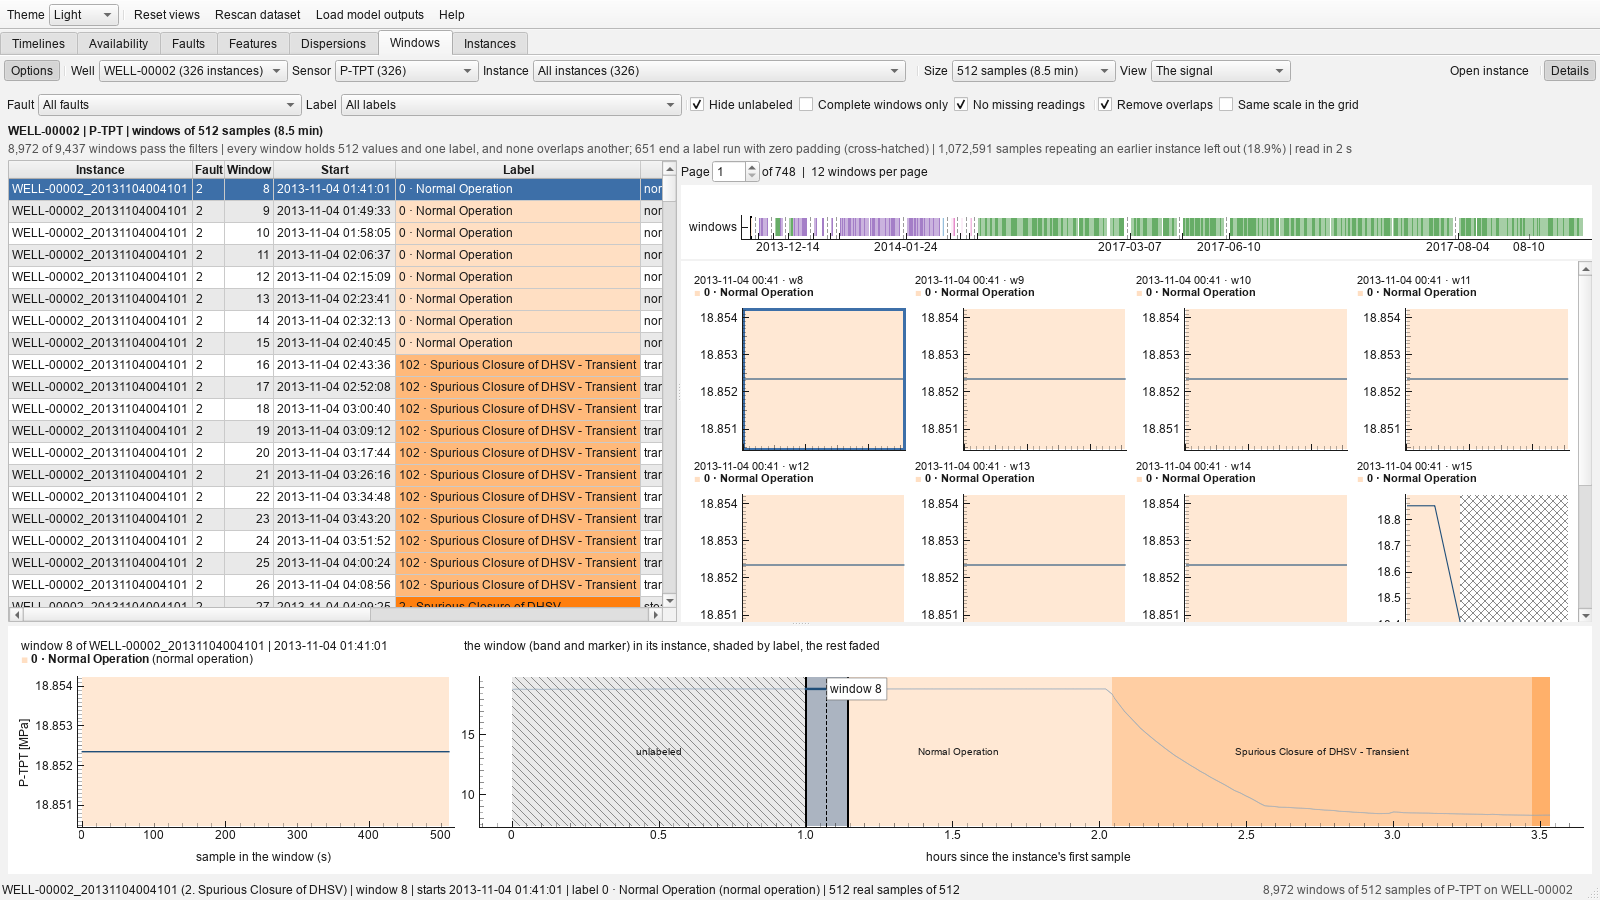
\includegraphics[width=\linewidth]{../assets/windows.png}
      \vskip 1.5mm
      \footnotesize
      \begin{itemize}
        \item \wspage{Windows}: one sensor of a well cut as a model reads it: 256, 512 or
          1024 samples a window, \textbf{one label each}, zero padded, no instant twice.
        \item A statistic per window and how well it \textbf{separates} normal from event
          windows; the largest well, 5.7 million samples, is cut in two seconds.
      \end{itemize}
    \end{column}
  \end{columns}
\end{frame}

% ---------------------------------------------------------------------------
\begin{frame}{Instances: every real instance on one plane}
  \begin{columns}[T]
    \begin{column}{0.6\textwidth}
      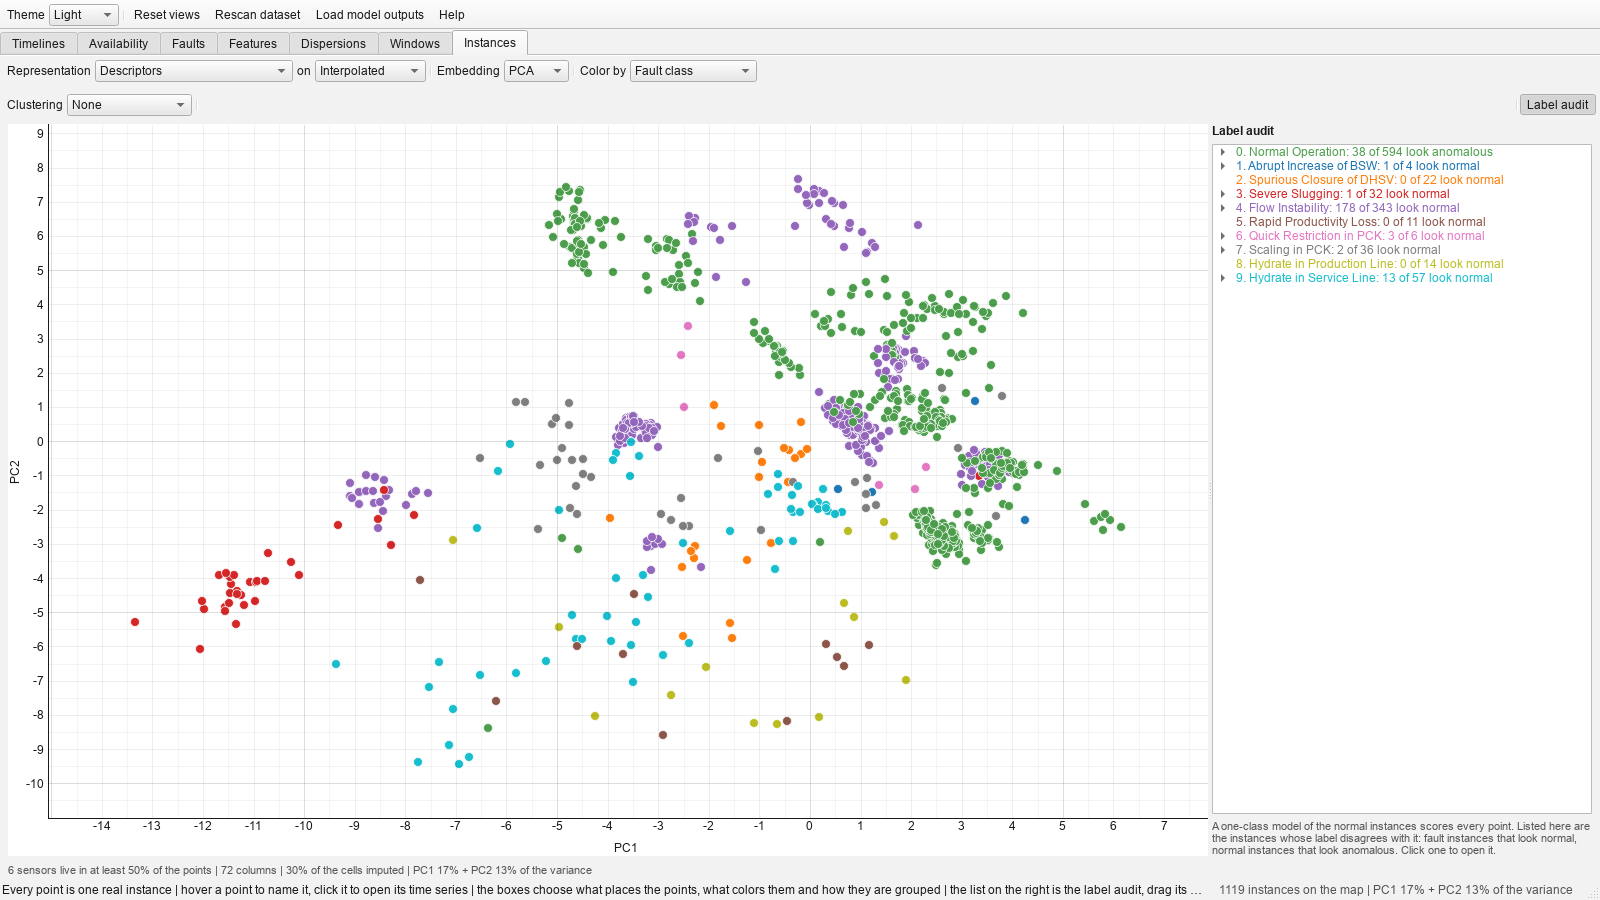
\includegraphics[width=\linewidth]{../assets/instances.png}
    \end{column}
    \begin{column}{0.38\textwidth}
      \footnotesize
      \begin{itemize}
        \item 1,119 points. An instance becomes a point by the \textbf{descriptors} of its
          sensors (moments, quantiles, autocorrelation time, signal-to-noise ratio,
          Gaussianity), by their shape alone, or by the Toolkit's \textbf{DTW} distance.
        \item \textbf{PCA}, \textbf{t-SNE} or \textbf{UMAP}; k-means, Gaussian mixture,
          agglomerative or DBSCAN, scored against the fault classes and against the wells:
          is it the event or the well that places an instance?
        \item \textbf{Typicality}, the distance to the medoid of the class, and a
          \textbf{label audit}: a one-class model of the normal instances lists the fault
          instances that look normal and the normal ones that look anomalous.
      \end{itemize}
    \end{column}
  \end{columns}
\end{frame}

% ---------------------------------------------------------------------------
\begin{frame}{The instance window: traces, labels, warnings}
  \begin{columns}[T]
    \begin{column}{0.6\textwidth}
      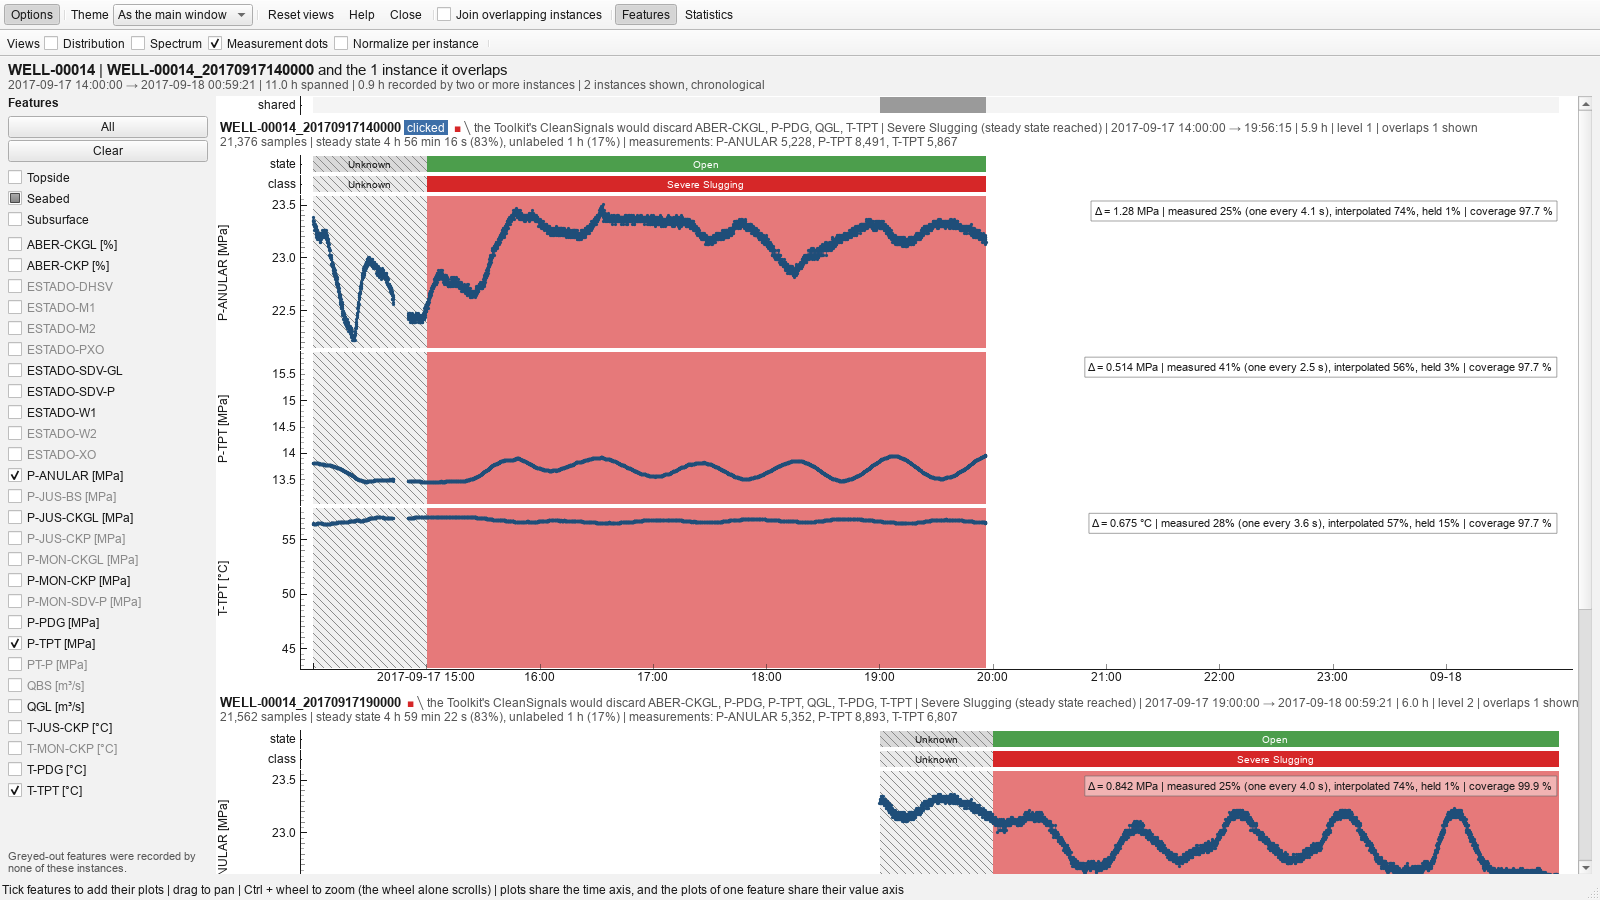
\includegraphics[width=\linewidth]{../assets/instance_window.png}
    \end{column}
    \begin{column}{0.38\textwidth}
      \footnotesize
      \begin{itemize}
        \item One block per instance, or per joined recording, on a \textbf{shared time
          axis}: the well status and the label as bands, a plot per sensor, the
          \textbf{measurements as dots} on the historian's line.
        \item Three warnings, from a survey of every real instance of 3W 2.0.0:
          \begin{itemize}
            \item \textcolor{ws3worange}{\textbf{amber}}: a reading no instrument could
              produce (a negative pressure, 30,000\,\textdegree C);
            \item \textcolor{ws3worange}{\textbf{amber, dashed}}: two pressures of one line
              out of order: \textbf{35 of 1,119} instances;
            \item \textcolor{red}{\textbf{red}}: a well status its valves contradict, Open
              with the wing valve closed: \textbf{41 of 1,119} instances.
          \end{itemize}
      \end{itemize}
    \end{column}
  \end{columns}
\end{frame}

% ---------------------------------------------------------------------------
\begin{frame}{What the viewer found: the historian's lines}
  \begin{columns}[T]
    \begin{column}{0.3\textwidth}\wsstat{6\,\%}{of the samples of 3W 2.0.0 are measurements}\end{column}
    \begin{column}{0.36\textwidth}\wsstat{55\,\% + 39\,\%}{interpolated and held between them by the PI historian}\end{column}
    \begin{column}{0.3\textwidth}\wsstat{33 s}{median interval between two measurements}\end{column}
  \end{columns}
  \vskip 4mm
  \begin{columns}[T]
    \begin{column}{0.54\textwidth}
      \footnotesize
      \begin{itemize}
        \item The dataset is sampled once a second, but the sensors were not read once a
          second: the historian \textbf{interpolated} between the values it archived. Melo
          saw it on WELL-00001 (doctoral thesis, section 4.2.5); the viewer tests every
          sample of every real instance.
        \item The rule: a sample equal to the one before is \textbf{held}; one collinear with
          both its neighbours is \textbf{interpolated}; everything else is a
          \textbf{measurement}. The tolerance, one part in a million, is read off the data.
        \item Every figure taken on the 1 Hz grid inherits the lines. Wherever the viewer
          shows one it says so, and offers it on the \textbf{measurements alone}.
      \end{itemize}
    \end{column}
    \begin{column}{0.44\textwidth}
      \footnotesize
      \setlength{\tabcolsep}{4pt}
      \begin{tabular}{@{}lrr@{}}
        \toprule
        T-JUS-CKP & on the grid & measured \\
        \midrule
        signal-to-noise ratio & 36,000 & 1.5 \\
        autocorrelation time & 7 min & 73 s \\
        \bottomrule
      \end{tabular}
      \vskip 2mm
      {\color{ws3wbrown} Where live, P-MON-CKP is read every 12 s, P-PDG every 13 s, T-TPT
      every 16 s, QGL every 21 s, P-TPT every 100 s, T-JUS-CKP every two minutes and
      P-ANULAR every four.\par}
    \end{column}
  \end{columns}
\end{frame}

% ---------------------------------------------------------------------------
\begin{frame}{Meeting the 3W Toolkit}
  \begin{columns}[T]
    \begin{column}{0.32\textwidth}
      \begin{block}{By rule}
        \footnotesize
        The Toolkit's \texttt{CleanSignals} decides, per instance and sensor, whether a
        signal is to be believed. The viewer holds exactly what the rule needs, so it
        applies it at no cost, lets its thresholds move, and marks every cell, bar and
        block the rule would discard, saying why.
      \end{block}
    \end{column}
    \begin{column}{0.32\textwidth}
      \begin{block}{By file}
        \footnotesize
        \textbf{Export file list} writes the instances a page has on show as the JSON of a
        \texttt{ParquetDatasetConfig} with \texttt{split="list"}, which the Toolkit loads
        with one line. The provenance is written beside it.
      \end{block}
    \end{column}
    \begin{column}{0.32\textwidth}
      \begin{block}{By model outputs}
        \footnotesize
        A folder: \texttt{model.json} and one parquet file per instance scored, with a
        \texttt{timestamp} index and a \texttt{label} column. The \textbf{agreement} with the
        experts' labels is drawn as a third band in the instance window, a bar color and a
        map coloring.
      \end{block}
    \end{column}
  \end{columns}
  \vskip 2mm
  \footnotesize
  \begin{itemize}
    \item The example shipped: a PCA control chart over the 319 real instances of four wells,
      one model per well. It agrees with the labels 98\,\% of the time on the normal
      instances and \textbf{between 100\,\% and 5\,\%} on the fault instances, the same event
      reading 100\,\% on one well and 5\,\% on another: the agreement says as much about a
      well's normal data as about the event.
    \item What cannot come back: the Toolkit's \texttt{predictions\_<timestamp>.csv} carries
      no instance and no instant, so nothing in it can be drawn onto the data. The folder
      format is the smallest one that says both.
  \end{itemize}
\end{frame}

% ---------------------------------------------------------------------------
\begin{frame}{What the viewer says back to 3W}
  \begin{columns}[T]
    \begin{column}{0.24\textwidth}
      \wsstat{41}{real instances whose well status the valves contradict}
      \wsstat{35}{real instances with two pressures of one line out of order}
      \wsstat{1.6\,\%}{unlabeled in the largest joined recording, a third apart}
    \end{column}
    \begin{column}{0.73\textwidth}
      \small
      \begin{itemize}
        \item \textbf{Labels worth a second look.} 41 instances are labeled Open while a
          valve of the production path reads closed or a crossover open, mostly for the
          whole recording; 35 carry a downstream pressure above its upstream one. Each is
          marked on the pages and one click from its trace.
        \item \textbf{Overlapping windows are one recording.} Joined, the largest group of
          3W 2.0.0 (71 windows over six days) keeps 1.6\,\% of its samples unlabeled where
          the windows apart left a third: the merged recording is what a model would train on.
        \item \textbf{The 1 Hz grid is the historian's, not the sensors'.} A spectrum, an
          autocorrelation or a signal-to-noise ratio taken on the grid describes the
          interpolation as much as the process; the measurements, 6\,\% of the samples, say
          which is which.
        \item \textbf{A model export that names the instance and the instant} can be drawn
          onto the data and compared with the experts, instance by instance. The viewer's
          folder format is one proposal for it.
      \end{itemize}
    \end{column}
  \end{columns}
\end{frame}

% ---------------------------------------------------------------------------
\begin{frame}{Try it}
  \begin{columns}[T]
    \begin{column}{0.64\textwidth}
      \begin{itemize}
        \item Python 3.11 or newer, \href{https://docs.astral.sh/uv/}{uv} and a local copy of
          3W 2.0.0; at least 1.4 GB of RAM. MIT license.
        \item The first launch scans the 1,119 instances in about 7 s and caches the
          catalogue; the heavier passes run once, behind a progress dialog, and are cached
          too.
        \item \texttt{backend} (pandas, numpy, pyarrow), \texttt{algorithms} (numpy) and
          \texttt{frontend} (PySide6, pyqtgraph); the heavier analyses are optional extras.
      \end{itemize}
      \begin{block}{From a shell}
        \footnotesize\ttfamily
        git clone https://github.com/Thiago-TP/3w-well-data-viewer\\
        cd 3w-well-data-viewer\\
        uv sync --all-extras\\
        uv run overlap-viewer --raw-dir /path/to/3W/dataset
      \end{block}
    \end{column}
    \begin{column}{0.33\textwidth}
      \centering
      \qrcode[height=30mm]{https://github.com/Thiago-TP/3w-well-data-viewer}
      \vskip 2mm
      \small\href{https://github.com/Thiago-TP/3w-well-data-viewer}{github.com/Thiago-TP/\\3w-well-data-viewer}\par
      \vskip 2mm
      {\scriptsize\color{ws3wbrown} Issues, questions and pull requests are welcome.\par}
    \end{column}
  \end{columns}
\end{frame}

% ---------------------------------------------------------------------------
\wsclosingframe[%
  github.com/Thiago-TP/3w-well-data-viewer\\
  thiagotomasdepaula@gmail.com]{Thank you!}

\end{document}
